\section{Implementation}
\label{sec:impl}

\begin{figure}
  \centering
  \begin{tikzpicture}
    \tikzstyle{node} = [
      rectangle,rounded corners,minimum width=1.5cm,minimum height=1cm,text centered,
      draw=black,fill=red!80,align=center,anchor=west,font=\footnotesize
    ];
    \tikzstyle{input} = [trapezium, trapezium left angle=70, trapezium right angle=110, minimum width=1.5cm, minimum height=1cm, text centered, draw=black, fill=blue!30,align=center,anchor=west,font=\footnotesize];

    \node (loop) [input] at (0,0) {Input loop\\expression};
    \node (loopy) [node,at={(loop.east)},xshift=.7cm] {Generate\\loopy kernel};
    \node (c) [node,at={(loopy.east)},xshift=.7cm] {Generate\\C code};
    \node (exe) [node,at={(c.east)},xshift=.7cm] {Compile\\binary};
    \node (do) [node,at={(exe.east)},xshift=.7cm] {Execute};

    \draw [-{stealth}] (loop) -- (loopy);
    \draw [-{stealth}] (loopy) -- (c);
    \draw [-{stealth}] (c) -- (exe);
    \draw [-{stealth}] (exe) -- (do);
    \draw [-{stealth},densely dashed] (loop) to [bend left=35]
      node[midway,above,align=center,font=\footnotesize] {Pass in data from\\loop expression} (do);
  \end{tikzpicture}
  \caption{The code generation and execution pipeline for a \pyop3 loop expression.}
  \label{fig:codegenproc}
\end{figure}

\begin{listing}
  \begin{minted}{c}
void do_loop(int ncells, double *dat0, double *dat1, int *map0) {
  double t0[CLOSURE_SIZE], t1[CLOSURE_SIZE];

  for (int c=0; c<ncells; ++c) {
    // Pack temporaries
    for (int p=0; p<CLOSURE_SIZE; ++p) {
      t0[p] = dat0[map0[c*CLOSURE_SIZE+p]];
      t1[p] = 0.0;
    }
    // Do the local computation
    kernel(t0, t1);
    // Now scatter the results
    for (int p=0; p<CLOSURE_SIZE; ++p) {
      dat1[map0[c*CLOSURE_SIZE+p]] += t1[p];
    }
  }
}
  \end{minted}
  \caption{
    Simplified version of code that would be generated by \pyop3 for the loop expression from Section~\ref{sec:impl_interface}.
    \clang{kernel} has access descriptors \py{READ} and \py{INC}, explaining the differing treatment for \clang{t0} and \clang{t1}.
    \clang{CLOSURE_SIZE} is an integer constant and would be known at compile-time.
  }
  \label{lst:basicloop}
\end{listing}

As discussed in Section~\ref{sec:stencillang}, existing stencil libraries may be classified according to whether or not they are aware of the mesh topology.
A library that is not `mesh-aware', for example \pyop2, can be more challenging to program in because responsibility for reasoning about the topology, including orientations, is passed to the user who has to construct the appropriate indirection maps to represent their mesh.
Composition of indirection maps is also difficult because of the loss of topological information.
Such difficulties can be avoided with a mesh-aware stencil library, but (usually) at the expense of relying upon a custom mesh abstraction implementation.
Writing mesh codes by hand is a non-trivial task requiring a significant amount of developer effort to maintain and introduce new features.
An in-house implementation will also never be able to compete with the feature set of a more general purpose mesh library (e.g. I/O, parallel decomposition, adaptive refinement) and will also suffer from poor interoperability with other packages.

In this work we attempt to bridge the gap between mesh-aware and mesh-oblivious stencil libraries by writing a new stencil library, \pyop3, that combines the advantages provided by mesh-aware frameworks with DMPlex, a mature, external mesh implementation (Section~\ref{sec:background_mesh_dmplex}).

\pyop3 is, somewhat obviously, heavily inspired by and based upon \pyop2, and hence much of its design represents either an incremental improvement on \pyop2, or is in fact directly lifted from it.
This report will make clear what parts of the design of \pyop3 are novel contributions and which are derived from \pyop2.

\subsection{Interface}
\label{sec:impl_interface}

\pyop3 is implemented as a \gls{dsl} embedded in Python.
As part of a larger script users create \textit{loop expressions}, prescribing the loops, local computations and stencil data access patterns in a manner resembling the algorithm's pseudocode.
These loop expressions are then parsed, compiled and executed by the \pyop3 backend.

To give an example, the syntax for a typical \gls{fem} residual assembly, where one loops over cells and computes using data in the cell's closure, would look something like:

\vspace{1em}
\begin{minipage}{\textwidth}
\begin{minted}[xleftmargin=4em]{python}
do_loop(
  c := mesh.cells.index,
  kernel(dat0[closure(c)], dat1[closure(c)])
)
\end{minted}
\end{minipage}
\vspace{1em}

Here the function \py{do_loop} declares and then executes the loop expression.
All loop expressions consist of:
1) an iteration set, here \py{mesh.cells}, and
2) a sequence of instructions to execute, here simply the single local kernel \py{kernel}.
\py{kernel} has type \py{LocalKernel} and consists of a \textit{loopy kernel} (Section~\ref{sec:impl_interface_codegen}) augmented with \textit{access descriptors} for each of its arguments.
Possible access descriptors are \py{READ}, \py{WRITE}, \py{RW}, \py{INC}, \py{MIN} and \py{MAX} and they are required to ensure that \pyop3 generates the right packing/unpacking code.
An example for a kernel with access descriptors \py{READ} and \py{INC} is shown in Listing~\ref{lst:basicloop}.
Lastly, the \py{dat{0,1}[closure(c)]} instructions indicate that \py{kernel} should be passed two contiguous arrays, each containing the \glspl{dof} associated with the closure of the current cell.
This last part is where the difference between the mesh-oblivious \pyop2 and the mesh-aware \pyop3 is stark.
In \pyop2 these closure maps would need to be computed in advance and passed in to the loop expression whereas \pyop3, being mesh-aware, is capable of reasoning about the mesh and automatically computing the right indirection maps.

Note that in this example, by using \py{do_loop}, we declare the loop expression and then \textit{immediately execute it}.
This is not always desired behaviour as, if the same loop expression is executed multiple times, one may want to have a \textit{persistent} loop expression to avoid some overhead.
Such expressions can easily be created by calling \py{expr = loop(...)}, and then executed with Python call syntax: \py{expr(*args, **kwargs)}.
This is discussed in more detail in Section~\ref{sec:impl_overhead}.

\subsubsection{Code generation}
\label{sec:impl_interface_codegen}

Having declared a loop expression, \pyop3 executes it by first lowering the expression through a sequence of intermediate representations, compiling to a binary, then running the code.

The target intermediate representation of \pyop3 is loopy~\cite{klocknerLooPyTransformationbased2014}, a polyhedral model inspired Python code generation library capable of generating code for multiple backends including CPUs and GPUs.
With loopy, the main entry point is, not dissimilarly to \pyop3, the declaration of a \py{LoopKernel} via the command \py{loopy.make_kernel}.
Once a \py{LoopKernel} has been created, loopy also provides a wealth of different code transformations such as loop tiling, vectorisation and loop-invariant code motion.

To construct such a kernel, the user needs to specify \textit{domains}, effectively loop extents, \textit{instructions} (e.g. \clang{x[i] += y[i]}) and \textit{arguments} representing kernel inputs.
For example, a simple loopy kernel could be created as follows:

\vspace{1em}
\begin{minipage}{\textwidth}
\begin{minted}[xleftmargin=2em]{python}
knl = loopy.make_kernel(
  "{ [i]: 0 <= i < n }",  # domains
  "y[i] = 2*x[i]",        # instructions
  [                       # arguments
    loopy.GlobalArg("x"),
    loopy.GlobalArg("y"),
    loopy.ValueArg("n"),
  ],
)
\end{minted}
\end{minipage}
\vspace{1em}

The role of \pyop3 in lowering to such a representation is therefore to determine the correct number and size of the iteration domains, and resolving the complex data access patterns required for multi-dimensional mesh data in order to emit the correct instructions.

Once \pyop3 has generated an appropriate loopy kernel, loopy is called upon to generate code in a low-level device-specific language (e.g. C for CPUs).
This code is then compiled by \pyop3 and executed.
A high-level overview of the code generation pathway is shown in Figure~\ref{fig:codegenproc} and an example of the sort of C code that would be emitted is shown in Listing~\ref{lst:basicloop}.

\subsubsection{Data types}

Just like \pyop2, \pyop3 has three main data types:
\py{Globals}, values shared across all processors;
\py{Dats}, vectors storing data associated with mesh points;
and \py{Mats}, matrices (usually sparse) representing interactions between mesh points.

The distribution of these parallel objects is discussed in Section~\ref{sec:impl_parallel}.

\subsection{A new abstraction for mesh data layouts}
\label{sec:impl_datalayout}

\begin{figure}
  \centering
  \begin{subfigure}[t]{0.48\textwidth}
    \centering
    \begin{tikzpicture}[y=-1cm,scale=.75]
      \begin{scope}[yshift=0cm]
        \fill[lightgray] (0,0) rectangle(6,1);
        \filldraw[draw=black, fill=white] (0.5,0) rectangle ++ (1,1);
        \filldraw[draw=black, fill=white] (1.5,0) rectangle ++ (1,1);
        \filldraw[draw=black, fill=white] (2.5,0) rectangle ++ (1,1);
        \filldraw[draw=black, fill=white] (3.5,0) rectangle ++ (1,1);
        \filldraw[draw=black, fill=white] (4.5,0) rectangle ++ (1,1);
        \node[at={(1,.5)}, ptlabel] {$i_0$};
        \node[at={(2,.5)}, ptlabel] {$i_1$};
        \node[at={(3,.5)}, ptlabel] {$i_4$};
        \node[at={(4,.5)}, ptlabel] {$i_5$};
        \node[at={(5,.5)}, ptlabel] {$i_9$};
        \draw (0,0) -- (6,0);
        \draw (0,1) -- (6,1);
      \end{scope}

      \begin{scope}[xshift=1.5cm,yshift=-2cm]
        \filldraw[draw=black, fill=white] (0,0) rectangle ++ (1,1);
        \filldraw[draw=black, fill=white] (1,0) rectangle ++ (1,1);
        \filldraw[draw=black, fill=white] (2,0) rectangle ++ (1,1);
        \node[at={(0.5,.5)}, ptlabel] {$d_0$};
        \node[at={(1.5,.5)}, ptlabel] {$d_1$};
        \node[at={(2.5,.5)}, ptlabel] {$d_2$};

        \draw (1,-1) -- (0,0);
        \draw (2,-1) -- (3,0);
      \end{scope}

      \node (nodeslabel) [ptlabel] at (7,.5) {Nodes};
      \node (dofslabel) [ptlabel] at (7,2.5) {\glspl{dof}};
    \end{tikzpicture}
    \caption{
      A typical \pyop2 \py{Dat} data layout for a \py{DataSet} with \py{dim} \py{(3,)}.
      Note that the nodes are unordered, since we are on an unstructured mesh, but that the \glspl{dof} are ordered.
    }
    \label{fig:vdat_pyop2}
  \end{subfigure}
  \hfill
  \begin{subfigure}[t]{0.48\textwidth}
    \centering
    \begin{tikzpicture}[y=-1cm,scale=.75]
      \begin{scope}[yshift=0cm]
        \fill[lightgray] (0,0) rectangle(6,1);
        \filldraw[draw=black, fill=white] (0.5,0) rectangle ++ (1,1);
        \filldraw[draw=black, fill=white] (1.5,0) rectangle ++ (1,1);
        \filldraw[draw=black, fill=white] (2.5,0) rectangle ++ (1,1);
        \filldraw[draw=black, fill=white] (3.5,0) rectangle ++ (1,1);
        \filldraw[draw=black, fill=white] (4.5,0) rectangle ++ (1,1);
        \node[at={(1,.5)}, ptlabel] {$c_5$};
        \node[at={(2,.5)}, ptlabel] {$v_1$};
        \node[at={(3,.5)}, ptlabel] {$e_4$};
        \node[at={(4,.5)}, ptlabel] {$e_5$};
        \node[at={(5,.5)}, ptlabel] {$c_9$};
        \draw (0,0) -- (6,0);
        \draw (0,1) -- (6,1);
      \end{scope}

      \begin{scope}[xshift=2cm,yshift=-2cm]
        \filldraw[draw=black, fill=white] (0,0) rectangle ++ (1,1);
        \filldraw[draw=black, fill=white] (1,0) rectangle ++ (1,1);
        \node[at={(0.5,.5)}, ptlabel] {$i_0$};
        \node[at={(1.5,.5)}, ptlabel] {$i_1$};

        \draw (.5,-1) -- (0,0);
        \draw (1.5,-1) -- (2,0);
      \end{scope}

      \begin{scope}[xshift=1cm,yshift=-4cm]
        \filldraw[draw=black, fill=white] (0,0) rectangle ++ (1,1);
        \filldraw[draw=black, fill=white] (1,0) rectangle ++ (1,1);
        \filldraw[draw=black, fill=white] (2,0) rectangle ++ (1,1);
        \node[at={(0.5,.5)}, ptlabel] {$d_0$};
        \node[at={(1.5,.5)}, ptlabel] {$d_1$};
        \node[at={(2.5,.5)}, ptlabel] {$d_2$};

        \draw (1,-1) -- (0,0);
        \draw (2,-1) -- (3,0);
      \end{scope}

      \node (pointslabel) [ptlabel] at (7,.5) {Points};
      \node (nodeslabel) [ptlabel] at (7,2.5) {Nodes};
      \node (dofslabel) [ptlabel] at (7,4.5) {\glspl{dof}};
    \end{tikzpicture}
    \caption{
      The equivalent \pyop3 data layout that is aware of the topology of the mesh.
      Note that the number of nodes per entity is not constant - here we indicate that there are 2 nodes per edge but this may differ for cells and vertices.
    }
    \label{fig:vdat_pyop3}
  \end{subfigure}
  \caption{Comparing the \gls{dof} layouts for a vector-valued \py{Dat} between \pyop2 (left) and \pyop3 (right).}
  \label{fig:vdat_comparison}
\end{figure}

\begin{figure}
  \centering
  \begin{subfigure}{.9\textwidth}
    \centering
    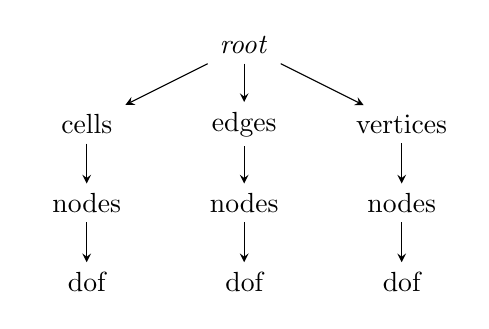
\begin{tikzpicture}
      \tikzstyle{node} = [minimum width=1.5cm,text centered,align=center];

      \node [node] (root) at (0,0) {\textit{root}};
      \node [node] (cells) at (-2,-1) {cells};
      \node [node] (edges) at (0,-1) {edges};
      \node [node] (verts) at (2,-1) {vertices};
      \node [node] (cnodes) at (-2,-2) {nodes};
      \node [node] (enodes) at (0,-2) {nodes};
      \node [node] (vnodes) at (2,-2) {nodes};
      \node [node] (cdofs) at (-2,-3) {\glspl{dof}};
      \node [node] (edofs) at (0,-3) {\glspl{dof}};
      \node [node] (vdofs) at (2,-3) {\glspl{dof}};

      \draw [-{stealth}] (root) -- (cells);
      \draw [-{stealth}] (root) -- (edges);
      \draw [-{stealth}] (root) -- (verts);
      \draw [-{stealth}] (cells) -- (cnodes);
      \draw [-{stealth}] (edges) -- (enodes);
      \draw [-{stealth}] (verts) -- (vnodes);
      \draw [-{stealth}] (cnodes) -- (cdofs);
      \draw [-{stealth}] (enodes) -- (edofs);
      \draw [-{stealth}] (vnodes) -- (vdofs);
    \end{tikzpicture}
    \caption{
      An example data layout tree.
      Each node in the tree, excluding \textit{root}, corresponds to a \pyop3 \py{AxisPart}.
    }
    \label{fig:vdat_tree}
  \end{subfigure}
  
  \vspace{1em}

  \begin{subfigure}{.9\textwidth}
    \begin{minted}[xleftmargin=4em,fontsize=\footnotesize]{python}
root = (
  MultiAxis()
  .add_part(AxisPart(ncells, id="cells"))
  .add_part(AxisPart(nedges, id="edges"))
  .add_part(AxisPart(nverts, id="verts"))
  .add_subaxis("cells", AxisPart(ncnodes, id="cnodes"))
  .add_subaxis("edges", AxisPart(nenodes, id="enodes"))
  .add_subaxis("verts", AxisPart(nvnodes, id="vnodes"))
  .add_subaxis("cnodes", AxisPart(ncdofs))
  .add_subaxis("enodes", AxisPart(nedofs))
  .add_subaxis("vnodes", AxisPart(nvdofs))
)
    \end{minted}
    \caption{
      \pyop3 code for constructing the tree structure shown above.
      \py{ncells}, \py{ncnodes} etc are integers and correspond to the number of entries for a given \py{AxisPart}.
    }
    \label{lis:demotreecode}
  \end{subfigure}
  \caption{Example hierarchical data layout for a \py{Dat} in \pyop3.}
  \label{fig:demotree}
\end{figure}

The additional flexibility \pyop3 has over \pyop2 is thanks to its novel abstraction for describing data layouts.

In \pyop2, data layouts are prescribed by associating data (i.e. \glspl{dof}) with \textit{sets}.
More precisely, they are described using a \py{DataSet}, which is formed by associating a \py{Set} with some \textit{local shape} (a tuple), termed its \py{dim}.
An example of this is shown in Figure~\ref{fig:vdat_pyop2}.
The \py{Set} here consists of the nodes in the mesh and the \py{dim} is \py{(3,)}, thus every node in the mesh stores 3 entries.

The fundamental idea behind \pyop3 is the observation that such a two-layered data layout is insufficient for fully describing the complexities of data living on an unstructured mesh; in particular, \textit{topological information is lost}.
Typical \py{Dats} in \pyop2 use the \textit{nodes} of the mesh to form the underlying \py{Set}.
Recalling from Section~\ref{sec:background_mesh} that the nodes of a mesh are associated with a particular topological entity (i.e. cells, edges, etc), using nodes as a basis for describing a data layout means that information about the topological entities these nodes come from is lost.
We claim that this `premature flattening' of the data layout is disadvantageous, and so \pyop3 aims for a more complete description of it.

In order to do so, \pyop3 replaces the two-layered \py{DataSet} abstraction with a hierarchical, tree-based data layout.
Each layer of the hierarchy (e.g. topological entities or nodes) is represented by a \py{MultiAxis} object, and to each \py{MultiAxis} is associated one or more \py{AxisParts}.
\py{AxisParts} correspond to a particular `class' of entity stored in the \py{MultiAxis} and, for instance, allow \pyop3 to differentiate between the cells, edges and vertices of the mesh.
An example of such a data layout is shown in Figure~\ref{fig:vdat_pyop3}.
Compared with the equivalent \pyop2 data layout in Figure~\ref{fig:vdat_pyop2}, one can immediately see how topological information is preserved via the addition of an extra ``Points" \py{MultiAxis}.
Since the mesh will have been renumbered to improve data locality (Section~\ref{sec:background_opt_locality}), entries from different \py{AxisParts} (cells, edges and vertices) need to be interleaved.

To construct the hierarchy, it is permitted to attach a new \py{MultiAxis} to each \py{AxisPart}.
The interface for this, and the resulting tree structure, is shown in Figure~\ref{fig:demotree}.

The hierarchical data layout system described here is similar to that used in Taichi~\cite{huTaichiLanguageHighperformance2019}, though Taichi does not support interleaving components of an axis as we do here.
It also has no support for distributed memory parallelism (see Section~\ref{sec:impl_parallel}).

\subsubsection{Addressing the inhomogeneous}

One major challenge presented by this new abstraction is that axes are no longer homogeneous.
Previously, in \pyop2, one could stride over a \py{Dat} with steps matching the size of its \py{dim}.
This is no longer possible since the strides for, say, the ``Points" \py{MultiAxis} in Figure~\ref{fig:vdat_pyop3} are not constant because the number of nodes stored can differ between topological entities.
Addressing individual topological entities therefore requires careful thought and in \pyop3 is separated into two phases:
1) entries in the data layout are addressed with \textit{typed multi-indices}, and
2) these multi-indices are composed with \textit{layout functions} to determine the correct offset into the data.

To start with the former, a typed multi-index is an object of the form $\big[(t_0, i_0), (t_2, i_2), \dots, (t_n, i_n)\big]$ where $t_x$ indicates the `type' of the index $i_y$.
To streamline the notation, rather than using a 2-tuple for each multi-index entry, they will instead be written in the form $\mathit{type}_{\mathit{index}}$ (e.g. $c_0$ might indicate the first entry of something with `cell' type).
With the typed multi-index, the type is used to select the correct \py{AxisPart} to use in the hierarchy, and the index indicates which entry of that type is to be selected.
To give an example, in order to correctly address the $d_0$ entry from Figure~\ref{fig:vdat_pyop3}, the multi-index $(e_4, i_0, d_0)$

Provided with a multi-index, we can now use the appropriate layout functions to determine the right memory address (offset) for the data.
In \pyop3, layout functions are simply functions that take one or more indices and return an offset value. 
For example, in the case of axes with constant strides, a layout function would be some affine function of the form \clang{offset = i*stride + step} (with \clang{i} the input index).
If the axis has non-constant strides then the layout function instead needs to be some sort of lookup table (i.e. \clang{offset = offsets[i]}).

Layout functions are associated with individual \py{AxisParts} and so the process of determining the correct offset for a given multi-index is as follows:
1) Each `type' in the multi-index is used to select a particular \py{AxisPart} in the hierarchy.
2) The index part of the multi-index entry is then passed to the layout function of the selected \py{AxisPart} to compute an offset value.
3) The offsets for each level of the hierarchy are added together, yielding the final memory address.

\subsubsection{Maps}
\label{sec:impl_datalayout_maps}

When we address some data, the provided data structure is associated with a particular multi-index.
When we directly address data structures, for example by doing the following:

\vspace{1em}
\begin{minipage}{\textwidth}
\begin{minted}[xleftmargin=4em]{python}
loop(c := mesh.cells.index, kernel(dat0[c]))
\end{minted}
\end{minipage}
\vspace{1em}

Then the multi-index getting used, \py{c}, is simply $[(C, i)]$.
This is a multi-index with only a single entry which targets all entries in the selected \py{AxisPart}, in this case all cells in the mesh.
We remark that only the outermost axes need be indexed - the inner axes (here nodes-per-cell and \glspl{dof}-per-node) are automatically included as full slices.

Since computing stencils requires the addressing of adjacent mesh points, we use \textit{maps} to describe which multi-indexes are required.
A map is defined as a \textit{function that accepts a multi-index and returns multiple multi-indices}:

As an example, for a mesh composed of triangles, the code

\begin{minted}[xleftmargin=4em]{python}
loop(c := mesh.cells.index, kernel(dat[closure(c)]))
\end{minted}

uses the $\closure$ DMPlex restriction operation to yield a map of the form

\begin{equation*}
  (c_i,)
  \to \big[
  (c_i,)
  ,\ (e_{j_0},) ,\ (e_{j_1},) ,\ (e_{j_2},)
  ,\ (v_{j_3},) ,\ (v_{j_4},) ,\ (v_{j_5},) \big] .
\end{equation*}

In other words, \py{closure(c)} yields, for every cell, 7 multi-indices pointing to the cell and the 6 incident edges and vertices.

In an analogous way to layout functions, maps can be implemented either using index functions (i.e. $e_0 = f(c_0)$), or lookup tables (\clang{e0 = map[c0]}) depending on whether or not there is structure to exploit in the data layout.
This enables, for example, the use of structured meshes without needing to incur the memory bandwidth cost of tabulating a lookup table.

The approach just described enables arbitrary map composition because maps now work in line with how DMPlex handles restrictions, namely functions between mesh points, rather than between points and nodes.
One can, for example, easily describe stencils over interior facets where the stencil is composed of \textit{the closure of the cells incident on a facet}, or, in DMPlex terminology, $\closure(\support(p))$:

\begin{minted}[xleftmargin=4em]{python}
do_loop(
  f := mesh.interior_facets.index,
  kernel(
    dat0[closure(support(f))],
    dat1[closure(support(f))]
  )
)
\end{minted}

Note that at present we restrict maps to only work for multi-indices where the `parent' indices are the same for the input and output indices.
This is sufficient for unstructured meshes but not for partially-structured meshes.
This is discussed in detail in Section~\ref{sec:future_partialstructure_maps}.

\subsubsection{Raggedness and sparsity}
\label{sec:impl_datalayout_ragged}

There are occasions where one needs a data structure where the extent of an inner dimension depends on an outer one.
This occurs for example in variable layer extruded meshes - the extent of the inner dimension (the columns) is dependent upon the mesh point in the base mesh.
To get this to work, \pyop3 needs to generate code that resembles:

\begin{minted}[xleftmargin=4em]{c}
for (int i=0; i<N; ++i)
  for (int j=0; j<nlayers[i]; ++j)
    ...
\end{minted}

Note how the inner loop extent is dependent upon the outer one via the \clang{nlayers} array.

In \pyop3, such a `ragged' data structure can be initialised in the following way:

\begin{minted}[xleftmargin=4em]{python}
nlayers = Dat(MultiAxis(AxisPart(N)), dtype=int)
root = (
  MultiAxis()
  .add_part(AxisPart(N, id="outer"))
  .add_subaxis("outer", AxisPart(nlayers))
)
\end{minted}

Instead of using a constant integer value to prescribe the extent of the inner \py{AxisPart}, another \py{MultiAxis}-using data structure is used instead.
Having extents also use \py{MultiAxes} is advantageous as the code generation procedure can be shared.

We can also use the same technique to generate code for maps with \textit{variable arity}.
An example of this would be for $\plexstar(p)$ for $p$ a vertex since the number of incident edges on a vertex is variable.
This is useful for patch-based computations (see Section~\ref{sec:future_patch}).

Although not yet implemented, it should be entirely possible to implement sparse data structures by making small extensions to the existing abstraction.
If we consider a sparse matrix compressed with compressed-sparse-row (CSR) format, the data layout is described using two arrays: the row and column indices.
This is very similar to our existing solution for ragged arrays except that we assume that the internal dimension is logically dense, and hence do not need to specify column indices.

It should be noted however that we are assuming that the matrix is local to a single processor.
Parallel sparse matrices are considerably more challenging to implement and so we defer the work to PETSc (see Section~\ref{sec:impl_parallel_matrices}).

\subsubsection{Orienting degrees-of-freedom}
\label{sec:impl_orientation}

% an advantage we have over Basix is we differentiate between nodes and dofs so can transform them
% separately. transformation matrices are very very small.

Having a hierarchical, `mesh-aware' data layout makes it straightforward to correctly handle orientations when packing stencils.
If the maps are augmented to also return relative orientation information (i.e. it identifies `flipped' edges etc), then the packing code can apply the correct transformations for each level of the \py{MultiAxis}.

As an example, we refer back to Figure~\ref{fig:orient_vector_flip}.
Noting that the data layout will decompose into points, nodes-per-point and \glspl{dof}-per-node, the transformation to canonical layout is done in two steps: permuting the nodes on the edge and flipping the individual \glspl{dof} such that they point in the right direction.
These operations map naturally to the different sub-axes of the data layout - the permutation applies to nodes and so can apply to the node axis, and the reflection applies to each \glspl{dof} individually and so can be applied to the \glspl{dof} axis.

\subsubsection{Data layout transformations}
\label{sec:impl_datalayoutopt}

\begin{figure}
  \centering
  \begin{subfigure}{.65\textwidth}
    \centering
    \begin{tikzpicture}[y=-1cm,scale=.75]
      \begin{scope}[xshift=3.25cm, yshift=0cm]
        \filldraw[draw=black, fill=blue!60] (0,0) rectangle (1,1);
        \filldraw[draw=black, fill=red!60] (1,0) rectangle (2,1);
        \node[at={(.5,.5)}, ptlabel] {$V_0$};
        \node[at={(1.5,.5)}, ptlabel] {$V_1$};
      \end{scope}

      \begin{scope}[yshift=-2cm]
        \begin{scope}[xshift=0cm]
          \fill[lightgray] (0,0) rectangle (4,1);
          \filldraw[draw=black, fill=white] (0.5,0) rectangle (1.5,1);
          \filldraw[draw=black, fill=white] (1.5,0) rectangle (2.5,1);
          \filldraw[draw=black, fill=white] (2.5,0) rectangle (3.5,1);
          \node[at={(1,.5)}, ptlabel] {$c_0$};
          \node[at={(2,.5)}, ptlabel] {$v_1$};
          \node[at={(3,.5)}, ptlabel] {$c_4$};
          \draw (0,0) -- (4,0);
          \draw (0,1) -- (4,1);
        \end{scope}

        \begin{scope}[xshift=4.5cm]
          \fill[lightgray] (0,0) rectangle (4,1);
          \filldraw[draw=black, fill=white] (0.5,0) rectangle (1.5,1);
          \filldraw[draw=black, fill=white] (1.5,0) rectangle (2.5,1);
          \filldraw[draw=black, fill=white] (2.5,0) rectangle (3.5,1);
          \node[at={(1,.5)}, ptlabel] {$c_0$};
          \node[at={(2,.5)}, ptlabel] {$v_1$};
          \node[at={(3,.5)}, ptlabel] {$c_4$};
          \draw (0,0) -- (4,0);
          \draw (0,1) -- (4,1);
        \end{scope}
      \end{scope}

      \draw (3.25,1) -- (0,2);
      \draw (4.25,1) -- (4,2);
      \draw (4.25,1) -- ({0+4.5},2);
      \draw (5.25,1) -- ({4+4.5},2);
    \end{tikzpicture}
    \caption{}
    \label{fig:mixedreorder_outer}
  \end{subfigure}
  %
  \begin{subfigure}{.3\textwidth}
    \centering
    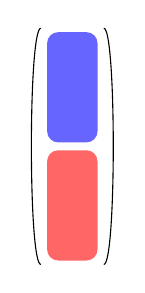
\begin{tikzpicture}[x=.8cm,y=-1cm]
      \draw (0,0) .. controls (-.2,0) and (-.2,3) .. (0,3);
      \draw (1,0) .. controls (1.2,0) and (1.2,3) .. (1,3);
      \filldraw [fill=blue!60,rounded corners,draw=none]
        (.1,.05) -- (.9,.05) -- (.9,1.45) -- (.1,1.45) -- cycle;
      \filldraw [fill=red!60,rounded corners,draw=none]
        (.1,1.55) -- (.9,1.55) -- (.9,2.95) -- (.1,2.95) -- cycle;
    \end{tikzpicture}
    \caption{}
    \label{fig:mixedreorder_outer_vec}
  \end{subfigure}

  \vspace{1em}
 
  \begin{subfigure}{.65\textwidth}
    \centering
    \begin{tikzpicture}[y=-1cm,scale=.75]
      \begin{scope}[xshift=0cm,yshift=0cm]
        \fill[lightgray] (0,0) rectangle (4,1);
        \filldraw[draw=black, fill=white] (0.5,0) rectangle (1.5,1);
        \filldraw[draw=black, fill=white] (1.5,0) rectangle (2.5,1);
        \filldraw[draw=black, fill=white] (2.5,0) rectangle (3.5,1);
        \node[at={(1,.5)}, ptlabel] {$c_0$};
        \node[at={(2,.5)}, ptlabel] {$v_1$};
        \node[at={(3,.5)}, ptlabel] {$c_4$};
        \draw (0,0) -- (4,0);
        \draw (0,1) -- (4,1);
      \end{scope}

      \begin{scope}[xshift=1cm, yshift=-2cm]
        \filldraw[draw=black, fill=blue!60] (0,0) rectangle (1,1);
        \filldraw[draw=black, fill=red!60] (1,0) rectangle (2,1);
        \node[at={(.5,.5)}, ptlabel] {$V_0$};
        \node[at={(1.5,.5)}, ptlabel] {$V_1$};
      \end{scope}

      \draw (1.5,1) -- (1,2);
      \draw (2.5,1) -- (3,2);
    \end{tikzpicture}
    \caption{}
    \label{fig:mixedreorder_inner}
  \end{subfigure}
  %
  \begin{subfigure}{.3\textwidth}
    \centering
    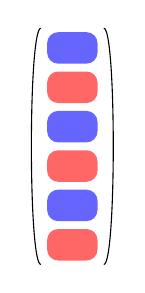
\begin{tikzpicture}[x=.8cm,y=-1cm]
      \tikzstyle{entry} = [rounded corners,draw=none];
      \tikzstyle{blue} = [entry,blue!60];
      \tikzstyle{red} = [entry,red!60];
      \draw (0,0) .. controls (-.2,0) and (-.2,3) .. (0,3);
      \draw (1,0) .. controls (1.2,0) and (1.2,3) .. (1,3);
      \filldraw [blue] (.1,.05) -- (.9,.05) -- (.9,.45) -- (.1,.45) -- cycle;
      \filldraw [red] (.1,.55) -- (.9,.55) -- (.9,.95) -- (.1,.95) -- cycle;
      \filldraw [blue] (.1,1.05) -- (.9,1.05) -- (.9,1.45) -- (.1,1.45) -- cycle;
      \filldraw [red] (.1,1.55) -- (.9,1.55) -- (.9,1.95) -- (.1,1.95) -- cycle;
      \filldraw [blue] (.1,2.05) -- (.9,2.05) -- (.9,2.45) -- (.1,2.45) -- cycle;
      \filldraw [red] (.1,2.55) -- (.9,2.55) -- (.9,2.95) -- (.1,2.95) -- cycle;
    \end{tikzpicture}
    \caption{}
    \label{fig:mixedreorder_inner_vec}
  \end{subfigure}
  \caption{}
  \label{fig:mixedreorder}
\end{figure}


With this decomposition of data layouts in a flexible, declarative hierarchy, it is now relatively straightforward to reason about making \textit{data layout transformations} to improve properties such as the effective working-set size (Section~\ref{sec:background_opt_locality}).

Some of the possible optimisations include:

\begin{paragraph}{Swapping axes}
\pyop3 makes it straightforward to swap a pair of \py{MultiAxis} such that the `inner' axis becomes the `outer' and vice versa.

An example of this is shown in Figure~\ref{fig:mixedreorder}.
Typically a `mixed' system like this - here formed of $V_0$ and $V_1$ - stores data in a blocked format (Figures~\ref{fig:mixedreorder_outer} and~\ref{fig:mixedreorder_outer_vec}).
This means that the \glspl{dof} corresponding to the same mesh point for $V_0$ and $V_1$ are very far apart in memory.
If they are both used in the local computation then this constitutes poor data locality.

To rectify the situation, we can, when applicable, permute the axes such that the mixed components are stored per mesh point, adjacent in memory.
An example of this is shown in Figures~\ref{fig:mixedreorder_inner} and~\ref{fig:mixedreorder_inner_vec}.
\end{paragraph}

\begin{paragraph}{Reordering data within axes}
Once the axes have been ordered in the most advantageous way, we can now begin to rearrange the entries in a \py{MultiAxis} to maximise locality.
In the context of meshes, these reorderings could correspond to, for example, an \gls{rcm} renumbering of the mesh entities or a different ordering of the elements up the columns of an extruded mesh.
In addition to improving locality, one can also perform these reorderings in order to allow for efficient subset queries.
Certain preconditioners require access to subsets of the mesh entities and the data layout can be modified so that the relevant \glspl{dof} are contiguous in memory.

To implement this reordering, \pyop3 simply requires that a different layout function be given to the respective \py{AxisParts}.
\end{paragraph}

\subsubsection{Other locality optimisations}

\pyop3's abstraction also enables code transformations such as vectorisation and tiling (Section~\ref{sec:background_opt_locality}).
Such optimisations are not data layout transformations, but transformations of the iteration set (i.e. the multi-index).
In both cases, the flat iteration over some axis needs to be transformed to a set of nested loops of the form

\begin{minipage}{\textwidth}
\begin{minted}[xleftmargin=4em]{c}
for (int i=0; i<NOUTER; ++i) {
  for (int j=0; j<NINNER; ++j) {
    int k = i*NINNER + j;
    ...
  }
}
\end{minted}
\end{minipage}

In the case of vectorisation, \clang{NINNER} would correspond to the length of the vector lanes of the CPU, and if tiling it would be tailored to its cache sizes.

It is valuable to note that, for unstructured meshes, tiling on its own is redundant as the amount of data shared between successive loops and prefetched by the hardware is already maximised by having an appropriate mesh numbering.
The optimisation only becomes valuable when combined with kernel fusion to produce time tiling.
Then the size of tiles should be chosen such that data required for both loops remains in cache between kernel invocations.

\subsubsection{Enabling new research}

In addition to the performance benefits espoused above, this new data layout abstraction should enable one to implement a number of new mathematical methods heretofore impossible to implement in \pyop2:

\begin{itemize}
  \item
    \textbf{p-adaptivity}
    In order to reduce the errors in a simulation, one may vary the polynomial degree of particular cells in a process known as p-adaptivity.
    It is tricky to automate a stencil code for looping over the mesh because:
    a) multiple local kernels are needed, one for each degree, and b) there are `hanging' \glspl{dof} at the boundaries between cells of differing degrees.
    Problem (a) is trivial to resolve in \pyop3.
    Rather than having a \py{MultiAxis} that is composed only of cells, edges and vertices (each a distinct \py{AxisPart}), additional \py{AxisParts} can be added such that mesh points of different degree are associated with a unique \py{AxisPart}.
    Problem (b) is more challenging to solve and requires the addition of \textit{constraints} to the abstraction.

  \item
    \textbf{Mixed meshes}
    A mixed mesh is a mesh composed of multiple different types of polytope (e.g. triangles and squares).
    Iterating over such a mesh poses the same fundamental problem as p-adaptivity: different local kernels are required depending on the polytope type.
    Since \pyop3 is `mesh-aware' and can reason about the different classes of mesh points, this problem becomes trivial.

  \item
    \textbf{Particle-in-cell methods}
    Particle-in-cell methods are a type of numerical method where the cells of a mesh are associated with a number of, possibly advecting, particles.
    Since the number of particles differs between cells, a variable arity map is required to address them (Section~\ref{sec:impl_datalayout_ragged}).
\end{itemize}

\subsection{Parallel design}
\label{sec:impl_parallel}

\begin{figure}
  \centering
  \begin{tikzpicture}[scale=1.3]
    % define styles
    \tkzSetUpStyle[draw=white,line width=5]{cell}
    \tkzSetUpStyle[line width=2,shorten >=.2cm,shorten <=.2cm]{edge}

    \tkzSetUpStyle[cell,fill=red!50]{p1cell}
    \tkzSetUpStyle[cell,fill=red!25]{p1cellhalo}
    \tkzSetUpStyle[edge,draw=red!80]{p1edge}
    \tkzSetUpStyle[draw=red!80,fill=red!80]{p1vert}
    \tkzSetUpStyle[cell,fill=blue!50]{p2cell}
    \tkzSetUpStyle[cell,fill=blue!25]{p2cellhalo}
    \tkzSetUpStyle[edge,draw=blue!80]{p2edge}
    \tkzSetUpStyle[draw=blue!80,fill=blue!80]{p2vert}

    \tkzSetUpStyle[densely dashed,shorten >=.1cm,shorten <=.1cm,line width=.5]{connector}

    % process 
    \begin{scope}
      % define nodes
      \tkzDefPoint(0,0){p1v0}
      \tkzDefPoint(.1,1.1){p1v1}
      \tkzDefPoint(0,1.9){p1v2}
      \tkzDefPoint(.2,3.1){p1v3}
      \tkzDefPoint(1.1,0){p1v4}
      \tkzDefPoint(1,1){p1v5}
      \tkzDefPoint(.9,2){p1v6}
      \tkzDefPoint(1,3){p1v7}
      \tkzDefPoint(2,0){p1v8}
      \tkzDefPoint(2.1,1){p1v9}
      \tkzDefPoint(2,2.1){p1v10}
      \tkzDefPoint(1.9,3.2){p1v11}
      \tkzDefPoint(3,-.1){p1v12}
      \tkzDefPoint(3.1,.9){p1v13}
      \tkzDefPoint(3,2.1){p1v14}
      \tkzDefPoint(3.1,3.1){p1v15}

      % cells
      \tkzDrawPolygon[p1cell](p1v0,p1v1,p1v4)
      \tkzDrawPolygon[p1cell](p1v1,p1v4,p1v5)
      \tkzDrawPolygon[p1cell](p1v1,p1v5,p1v6)
      \tkzDrawPolygon[p1cell](p1v1,p1v2,p1v6)
      \tkzDrawPolygon[p1cell](p1v2,p1v3,p1v6)
      \tkzDrawPolygon[p1cell](p1v3,p1v6,p1v7)
      \tkzDrawPolygon[p1cell](p1v4,p1v8,p1v9)
      \tkzDrawPolygon[p1cell](p1v4,p1v5,p1v9)
      \tkzDrawPolygon[p1cell](p1v5,p1v9,p1v10)
      \tkzDrawPolygon[p1cell](p1v5,p1v6,p1v10)
      \tkzDrawPolygon[p1cell](p1v6,p1v7,p1v10)
      \tkzDrawPolygon[p1cell](p1v7,p1v10,p1v11)
      \tkzDrawPolygon[p1cell](p1v8,p1v9,p1v12)
      \tkzDrawPolygon[p2cellhalo](p1v9,p1v12,p1v13)
      \tkzDrawPolygon[p2cellhalo](p1v9,p1v13,p1v14)
      \tkzDrawPolygon[p1cell](p1v9,p1v10,p1v14)
      \tkzDrawPolygon[p2cellhalo](p1v10,p1v14,p1v15)
      \tkzDrawPolygon[p1cell](p1v10,p1v11,p1v15)

      % edges
      \tkzDrawSegments[p1edge](p1v4,p1v5 p1v5,p1v6 p1v6,p1v7)
      \tkzDrawSegments[p1edge](p1v8,p1v9 p1v9,p1v10 p1v10,p1v11)
      \tkzDrawSegments[p2edge,opacity=.5](p1v12,p1v13 p1v13,p1v14 p1v14,p1v15)

      \tkzDrawSegments[p1edge](p1v0,p1v4 p1v4,p1v8)
      \tkzDrawSegments[p1edge](p1v1,p1v5 p1v5,p1v9)
      \tkzDrawSegments[p1edge](p1v2,p1v6 p1v6,p1v10)
      \tkzDrawSegments[p1edge](p1v3,p1v7 p1v7,p1v11 p1v11,p1v15)
      \tkzDrawSegments[p2edge,opacity=.5](p1v8,p1v12 p1v9,p1v13 p1v10,p1v14)

      \tkzDrawSegments[p1edge](p1v1,p1v4 p1v1,p1v6 p1v3,p1v6)
      \tkzDrawSegments[p1edge](p1v4,p1v9 p1v5,p1v10 p1v7,p1v10)
      \tkzDrawSegments[p2edge,opacity=.5](p1v9,p1v12 p1v9,p1v14 p1v10,p1v15)  % mimics process 2

      % vertices
      % \tkzDrawPoints[p1vert](p1v0,p1v1,p1v2,p1v3,p1v4,p1v5,p1v6,p1v7)  % core
      \tkzDrawPoints[p1vert,size=5](p1v4,p1v5,p1v6,p1v7)  % core
      % \tkzDrawPoints[p1vert,diamond,size=6](p1v8,p1v9,p1v10,p1v11)  % owned
      \tkzDrawPoints[p1vert,diamond,size=6](p1v8,p1v9,p1v11)  % owned
      \tkzDrawPoints[p1vert,diamond,size=6,draw=black](p1v10)  % owned
      \tkzDrawPoints[p2vert,diamond,opacity=.5,size=6](p1v12,p1v13,p1v14,p1v15)

      % debugging
      % \tkzLabelPoints[anchor=south,font=\tiny](p1v0,p1v1,p1v2,p1v3,p1v4,p1v5,p1v6,p1v7,p1v8,p1v9,p1v10,p1v11,p1v12,p1v13,p1v14,p1v15)

      % draw a sample patch
      \tkzDefShiftPoint[p1v7](-.2,.2){p1v7patch}
      \tkzDefShiftPoint[p1v11](0,.2){p1v11patch}
      \tkzDefShiftPoint[p1v15](.2,.2){p1v15patch}
      \tkzDefShiftPoint[p1v14](.2,-.1){p1v14patch}
      \tkzDefShiftPoint[p1v9](.1,-.2){p1v9patch}
      \tkzDefShiftPoint[p1v5](-.2,-.2){p1v5patch}
      \tkzDefShiftPoint[p1v6](-.2,0){p1v6patch}
      \filldraw[draw=black,fill=black,fill opacity=.1,rounded corners=3]
      % \filldraw[draw=none,fill=blue,fill opacity=.4,rounded corners=2]
      % \filldraw[pattern={Hatch[distance=3mm,angle=45]},draw=black,rounded corners=2]
        (p1v7patch) -- (p1v11patch) -- (p1v15patch) -- (p1v14patch) -- (p1v9patch) --
        (p1v5patch) -- (p1v6patch) -- cycle;
      % \draw (p1v10) circle [radius=5pt];
      % \tkzDrawPoint[size=1pt](p1v10)

      % label "core" and "owned"
      \node (p1core) [inner sep=0pt,xshift=-20pt,yshift=20pt] at (p1v7) {\footnotesize core};
      \node (p1owned) [inner sep=0pt,xshift=-10pt,yshift=20pt] at (p1v11) {\footnotesize owned};
      \draw [-{stealth},shorten >=4pt,shorten <=2pt] (p1core.south) -- (p1v7.north);
      \draw [-{stealth},shorten >=4pt,shorten <=2pt] (p1owned.south) -- (p1v11.north);
    \end{scope}

    % process 2
    \begin{scope}[xshift=5cm]
      % define nodes
      \tkzDefPoint(0,0){p2v0}
      \tkzDefPoint(.1,1){p2v1}
      \tkzDefPoint(0,2.1){p2v2}
      \tkzDefPoint(-.1,3.2){p2v3}
      \tkzDefPoint(1,-.1){p2v4}
      \tkzDefPoint(1.1,.9){p2v5}
      \tkzDefPoint(1,2.1){p2v6}
      \tkzDefPoint(1.1,3.1){p2v7}
      \tkzDefPoint(2,-.1){p2v8}
      \tkzDefPoint(2,1.1){p2v9}
      \tkzDefPoint(2.1,2){p2v10}
      \tkzDefPoint(2,2.9){p2v11}
      \tkzDefPoint(3,.1){p2v12}
      \tkzDefPoint(3.1,1){p2v13}
      \tkzDefPoint(2.9,2){p2v14}
      \tkzDefPoint(2.9,3.1){p2v15}

      % cells
      \tkzDrawPolygon[p1cellhalo](p2v0,p2v1,p2v4)
      \tkzDrawPolygon[p2cell](p2v1,p2v4,p2v5)
      \tkzDrawPolygon[p2cell](p2v1,p2v5,p2v6)
      \tkzDrawPolygon[p1cellhalo](p2v1,p2v2,p2v6)
      \tkzDrawPolygon[p2cell](p2v2,p2v6,p2v7)
      \tkzDrawPolygon[p1cellhalo](p2v2,p2v3,p2v7)
      \tkzDrawPolygon[p2cell](p2v4,p2v5,p2v8)
      \tkzDrawPolygon[p2cell](p2v5,p2v8,p2v9)
      \tkzDrawPolygon[p2cell](p2v5,p2v6,p2v9)
      \tkzDrawPolygon[p2cell](p2v6,p2v9,p2v10)
      \tkzDrawPolygon[p2cell](p2v6,p2v10,p2v11)
      \tkzDrawPolygon[p2cell](p2v6,p2v7,p2v11)
      \tkzDrawPolygon[p2cell](p2v8,p2v9,p2v12)
      \tkzDrawPolygon[p2cell](p2v9,p2v12,p2v13)
      \tkzDrawPolygon[p2cell](p2v9,p2v10,p2v13)
      \tkzDrawPolygon[p2cell](p2v10,p2v13,p2v14)
      \tkzDrawPolygon[p2cell](p2v10,p2v14,p2v15)
      \tkzDrawPolygon[p2cell](p2v10,p2v11,p2v15)

      % edges
      \tkzDrawSegments[p1edge,opacity=.5](p2v0,p2v1 p2v1,p2v2 p2v2,p2v3)
      \tkzDrawSegments[p2edge](p2v4,p2v5 p2v5,p2v6 p2v6,p2v7)
      \tkzDrawSegments[p2edge](p2v8,p2v9 p2v9,p2v10 p2v10,p2v11)

      \tkzDrawSegments[p2edge](p2v0,p2v4 p2v4,p2v8 p2v8,p2v12)
      \tkzDrawSegments[p2edge](p2v1,p2v5 p2v5,p2v9 p2v9,p2v13)
      \tkzDrawSegments[p2edge](p2v2,p2v6 p2v6,p2v10 p2v10,p2v14)
      \tkzDrawSegments[p2edge](p2v7,p2v11 p2v11,p2v15)
      \tkzDrawSegments[p1edge,opacity=.5](p2v3,p2v7)

      \tkzDrawSegments[p2edge](p2v1,p2v4 p2v1,p2v6 p2v2,p2v7)
      \tkzDrawSegments[p2edge](p2v5,p2v8)
      \tkzDrawSegments[p2edge](p2v6,p2v9)
      \tkzDrawSegments[p2edge](p2v6,p2v11)
      \tkzDrawSegments[p2edge](p2v9,p2v12 p2v10,p2v13 p2v10,p2v15)

      % vertices
      \tkzDrawPoints[p2vert,size=5](p2v8,p2v9,p2v10,p2v11)  % core
      \tkzDrawPoints[p2vert,diamond,size=6](p2v4,p2v5,p2v6,p2v7)  % owned
      \tkzDrawPoints[p1vert,diamond,size=6,opacity=.5](p2v0,p2v1,p2v2,p2v3)  % halo

      % label "core" and "owned"
      \node (p2core) [inner sep=0pt,xshift=15pt,yshift=20pt] at (p2v11) {\footnotesize core};
      \node (p2owned) [inner sep=0pt,xshift=10pt,yshift=20pt] at (p2v7) {\footnotesize owned};
      \draw [-{stealth},shorten >=4pt,shorten <=2pt] (p2core.south) -- (p2v11.north);
      \draw [-{stealth},shorten >=4pt,shorten <=2pt] (p2owned.south) -- (p2v7.north);

      % debugging
      % \tkzLabelPoints[anchor=south,font=\tiny](p2v0,p2v1,p2v2,p2v3,p2v4,p2v5,p2v6,p2v7,p2v8,p2v9,p2v10,p2v11,p2v12,p2v13,p2v14,p2v15)
    \end{scope}

    % connect (sample of) equivalent points
    \draw [-{stealth},connector,shorten >=4pt,shorten <=4pt] (p1v11) to [bend left=45] (p2v3);
    \draw [{stealth}-,connector,shorten >=4pt,shorten <=4pt] (p1v15) to [bend left=45] (p2v7);
    \draw [-{stealth},connector,shorten >=4pt,shorten <=4pt] (p1v8) to [bend right=45] (p2v0);
    \draw [{stealth}-,connector,shorten >=4pt,shorten <=4pt] (p1v12) to [bend right=45] (p2v4);

    % label processes
    \node (p1name) at (1.5,4.2) {Process 1};
    \node (p2name) at (6.5,4.2) {Process 2};
  \end{tikzpicture}
  \caption{
    An example mesh distributed between two processes (red and blue).
    The mesh is intended for vertex patches (shaded) and so the overlap is chosen such that all required \glspl{dof} are stored locally.
    `Core' vertices are stored as circles and `owned' as diamonds.
    The direction of halo exchanges is indicated by the arrows.
  }
  \label{fig:halos}
\end{figure}

At present, \pyop3 implements an identical approach to distributed computing as \pyop2: \py{Globals}, \py{Dats} and \py{Mats} are distributed between processes using MPI parallelism; a hybrid model including shared memory (e.g. OpenMP) is not used.

To begin with, distribution of \py{Globals} is trivial.
They represent globally consistent values and so consensus between processes is reached via global reductions.

\subsubsection{Dats}

In stark contrast, \py{Dats} are distributed in a much more interesting manner.
Each process has a set of \glspl{dof} that it `owns' plus a `halo' region containing adjacent \glspl{dof} required for computations over the owned points.
Also, the points \textit{in the iteration set} belonging to the process are classified into \textit{core} and \textit{owned} sets.
Core points are those where a computation can be executed without requiring an up-to-date set of halo entries and owned points are those where it is required.
Classifying the points into these two categories allows \pyop3 to interleave computation and communication: \textit{core} points can be computed over while the halo exchanges required for \textit{owned} points are in-flight.

This situation is illustrated in Figure~\ref{fig:halos}.
It shows a mesh distributed across two processes.
Points `belonging' to a process are shown in red and blue respectively and the halo values are shown in the appropriate colour for each.

In this example, the stencil getting used in the iteration is the closure of the patch of cells around a vertex (i.e. $\closure(\plexstar(v))$).
Since this constitutes a fairly large stencil, the halos have to be correspondingly larger to contain all of the values required by the vertices belonging to the process.

In the figure, \textit{core} vertices are shown as circles and \textit{owned} as diamonds.
One can see that stencils involving the \textit{core} vertices can be executed without the need for a halo exchange (all points in the stencil are the same colour/on the same process as the vertex itself).
Similarly, the patches around \textit{owned} vertices contain at least one mesh point belonging to another process and hence a halo exchange is required.

In this example we have chosen to demonstrate mesh partioning using halos of the smallest possible size.
This is frequently desirable, smaller halos mean less data is transferred, but not in every case.
If the cost of computing the stencils is smaller than the cost of data movement one may want a larger halo.
This gains in terms of reduced data movement, but leads to each process performing some extra computations inside the wider halo region.
Such a strategy is not currently implemented in \pyop2 or \pyop3, but it has been pursued in the past~\cite{luporiniAutomatedTilingUnstructured2019}.

\subsubsection{Mats}
\label{sec:impl_parallel_matrices}

\pyop3 currently\footnotemark relies on PETSc to provide routines for matrix insertion.
In parallel, PETSc distributes the data by partitioning the rows between processes.
\footnotetext{We would like to have a more unified abstraction for \py{Globals}, \py{Dats} and \py{Mats} but this is very preliminary work and not discussed in this report.}

\subsubsection{Scaling}

Weak-scaling is an appropriate metric to evaluate the parallel communication design patterns described above, and in fact both PyOP2 and PETSc have been demonstrated to have good weak-scaling performance~\cite{rathgeberFiredrakeAutomatingFinite2016}. % FIXME include PETSc citation
Strong-scaling is a different story and is addressed in Section~\ref{sec:impl_overhead}.

\subsection{Avoiding Python overhead}
\label{sec:impl_overhead}

Python is the language of choice for \pyop3 for a number of compelling reasons.
Dynamic typing and being interpreted instead of compiled makes it very fast for users to prototype code.
It also has great syntax, especially for domain-specific languages.
User scripts are frequently shorter than 100 lines of code.

The primary complaint levelled at Python is that it is much slower, often by a factor of 100, than a compiled language like C or Fortran.
In general this issue is not important in code generation frameworks like \pyop3 and Firedrake since the performance critical parts of the code - the `hot loops' - are actually compiled C code and just as fast as code that is written by hand.
The fact that the rest of the library is written in Python does not matter as only a tiny fraction of the programs runtime is spent there.

However, there is one significant occasion where this claim falls down, and our choice of Python as language causes trouble: in the strong-scaling limit (Section~\ref{sec:background_perf_efficiency}).
In this limit the problem occupying the `hot loops' is `small' and hence completes very quickly.
This means that more time is spent in the Python interpreter which is slow.
Firedrake has been observed to have poor strong-scaling behaviour~\cite{changComparativeStudyFinite2018}\footnote{The results shown in this paper are exaggerated. We found that it was possible to substantially improve scaling performance with a few minor code modifications.}.

The solution to this issue is simple: spend less time in the Python layer.
This can be accomplished in two ways: write the new hot loops in a compiled language, possibly via code generation, or avoid doing extra work in Python by applying judicious caching.
Doing the former is somewhat trivial and will not be discussed here.
We will instead focus on achieving performant caching solutions in \pyop3.

Since the principle object in \pyop3 is the loop expression, we will only discuss this.
As mentioned in Section~\ref{sec:impl_jit}, one way to execute a loop expression is to use the function \py{do_loop(...)}.
This instantiates a new loop expression and then executes it.
While concise, this function is not suitable if one wants to execute an identical loop expression repeatedly because, at each iteration, the expression needs to be hashed prior to being able to use any internal caching (e.g. for the generated code).

To resolve this particular issue one can create a persistent loop expression via the command \py{expr = loop(...)} (taking the same arguments as \py{do_loop(...)}), which can then be executed with \py{expr.apply()}.
Having a persistent expression means that it can be hashed once and any cached objects may be directly accessed.

At this point, however, care needs to be taken with the data structures involved.
The loop expression is created using `heavy' data-carrying objects like \py{Dats} and \py{Mats} and so indiscriminate caching of the expression would result in a memory leak.
Along similar lines, it is also difficult to `swap out' data structures in the loop expression without requiring the instantiation of a brand new expression.
In other words, if one wanted to, say, execute the same loop expression but write the output to a different data structure, then this would require the creation of a new loop expression and reincur the, totally unnecessary, cost of hashing the expression.

To resolve this, \pyop3 loop expressions will store \textit{weak references} to the data structures in the loop expression and \py{expr.apply} will take optional keyword arguments to swap out the data structures as appropriate (e.g. \py{expr.apply(out=mynewdat)}).
In Python, weak references are references to objects that do not increase their \textit{reference count}.
This prevents memory leaks because the lifetime of a data structure will only be tied to its own scope, they will still be cleaned up even if they are referenced in a cached loop expression.
